% Chapter 12: Fourier Neural Operators (FNO) from Scratch
% Part II of the book.

\chapter{Fourier Neural Operators (FNO) from Scratch}
\label{ch:part2-fourier-neural-operators-fno-from-scratch}
\label{sec:fno_impl}
% -----------------------------------------------------------------------------

\chapref{ch:part1-the-fourier-neural-operator-spectral-theor} ends with a layer,
\eqref{eq:fno_layer}, and a bound on how far a stack of such layers can sit from
a target operator. Neither object runs. Between the display and a training loop
lie three questions the theorem does not ask: which entries of a discrete
transform correspond to which wavenumbers of the continuum, and what the
transform's normalization does to the learned multiplier; how the conjugacy
constraint \eqref{eq:ch05-reality} is enforced without storing twice the
parameters it needs; and what one layer costs, in floating-point operations and
in the bytes of device memory a batch must occupy. This chapter answers all
three by writing the two-dimensional spectral convolution out once in symbols
and once in PyTorch, and by holding the two accounts side by side.

The \textbf{Fourier neural operator} (FNO)~\cite{li2021fourier} parameterizes
non-local integral kernels directly in frequency space.
\index{Fourier neural operator!PyTorch implementation}
Developing it from first principles is worth the effort even for a reader who
will import a library model, because the failure modes of a spectral layer --- a
mode budget that silently overlaps itself, a weight array that no longer matches
the grid it is applied to, a frequency tensor that exhausts memory before the
first epoch ends --- are legible only to someone who has written the slicing by
hand.

Two kinds of background are assumed. The first is programming in PyTorch: the
\texttt{nn.Module} and \texttt{nn.Parameter} API and indexing by slices,
together with the channel-first tensor layout of
\chapref{ch:part2-the-practitioner-s-paradigm-infinite-dimen},
$X \in \mathbb{R}^{B \times C \times N_1 \times \cdots \times N_d}$.
\index{tensor layout!channel-first}
The second is the vocabulary of running on a graphics processing unit (GPU):
placing a tensor on a device, the cuDNN (CUDA Deep Neural Network) library's
batched convolution kernels, single precision (fp32) versus bfloat16, and the
fact that a forward pass retains its intermediates for automatic differentiation
and therefore pays for them twice.
\index{graphics processing unit (GPU)}
The route taken is linear. The first section walks the arithmetic of a single
spectral convolution and its listing; the second tallies what that layer costs
and how it fails; the third assembles the complete model around it; the fourth
sets all three against the official \texttt{neuraloperator} library. The chapter
fixes itself to two spatial dimensions on purpose --- the
one-dimensional and three-dimensional variants change the number of transformed
axes and the number of retained corners, not the arithmetic --- and leaves
scheduling, precision policy, and rollout to
\chapref{ch:part2-training-regimes-optimization-and-failure-}.

% -----------------------------------------------------------------------------
\section{Detailed Spectral Convolution Arithmetic}
\label{sec:ch23-spectral-arithmetic}
% -----------------------------------------------------------------------------

Figure~\ref{fig:fno_spectral} diagrams the tensor dataflow through a 2D spectral
convolution layer, and reading it stage by stage yields the claims about shapes
and roles that the code must realize. An input tensor of shape
$(B, C_{\text{in}}, H, W)$ splits into two paths. The upper path is a pointwise
linear map $W$, drawn as
$\operatorname{Conv2d}(C_{\text{in}}, C_{\text{out}}, k{=}1)$, whose output is
$(B, C_{\text{out}}, H, W)$: it mixes channels at a fixed grid point and touches
no other point. The lower path is the global spectral convolution
$\mathcal{K}$, drawn as three boxes. The figure labels the first with
$(B, C_{\text{in}}, H, \tfrac{W}{2}+1)$ complex entries and the third with the
real space $(B, C_{\text{out}}, H, W)$, but it states no shape for the middle
stage, only the shape of $R_\phi$ itself. That shape has to be read off the
code: it is $(B, C_{\text{out}}, H, \tfrac{W}{2}+1)$, the same half-spectrum
with the channel axis moved from $C_{\text{in}}$ to $C_{\text{out}}$, and it is
the shape of \texttt{out\_ft} in Listing~\ref{lst:ch23-spectral-conv2d}. The two
paths are then summed and
passed through the activation $\sigma$. The conclusion the figure carries is
architectural: nothing on the lower path couples two frequencies, so all spatial
communication is performed by the transform pair and all spatial locality by $W$,
and the learned array performs neither.
\index{local bypass convolution}

\begin{figure}[htbp]
\centering
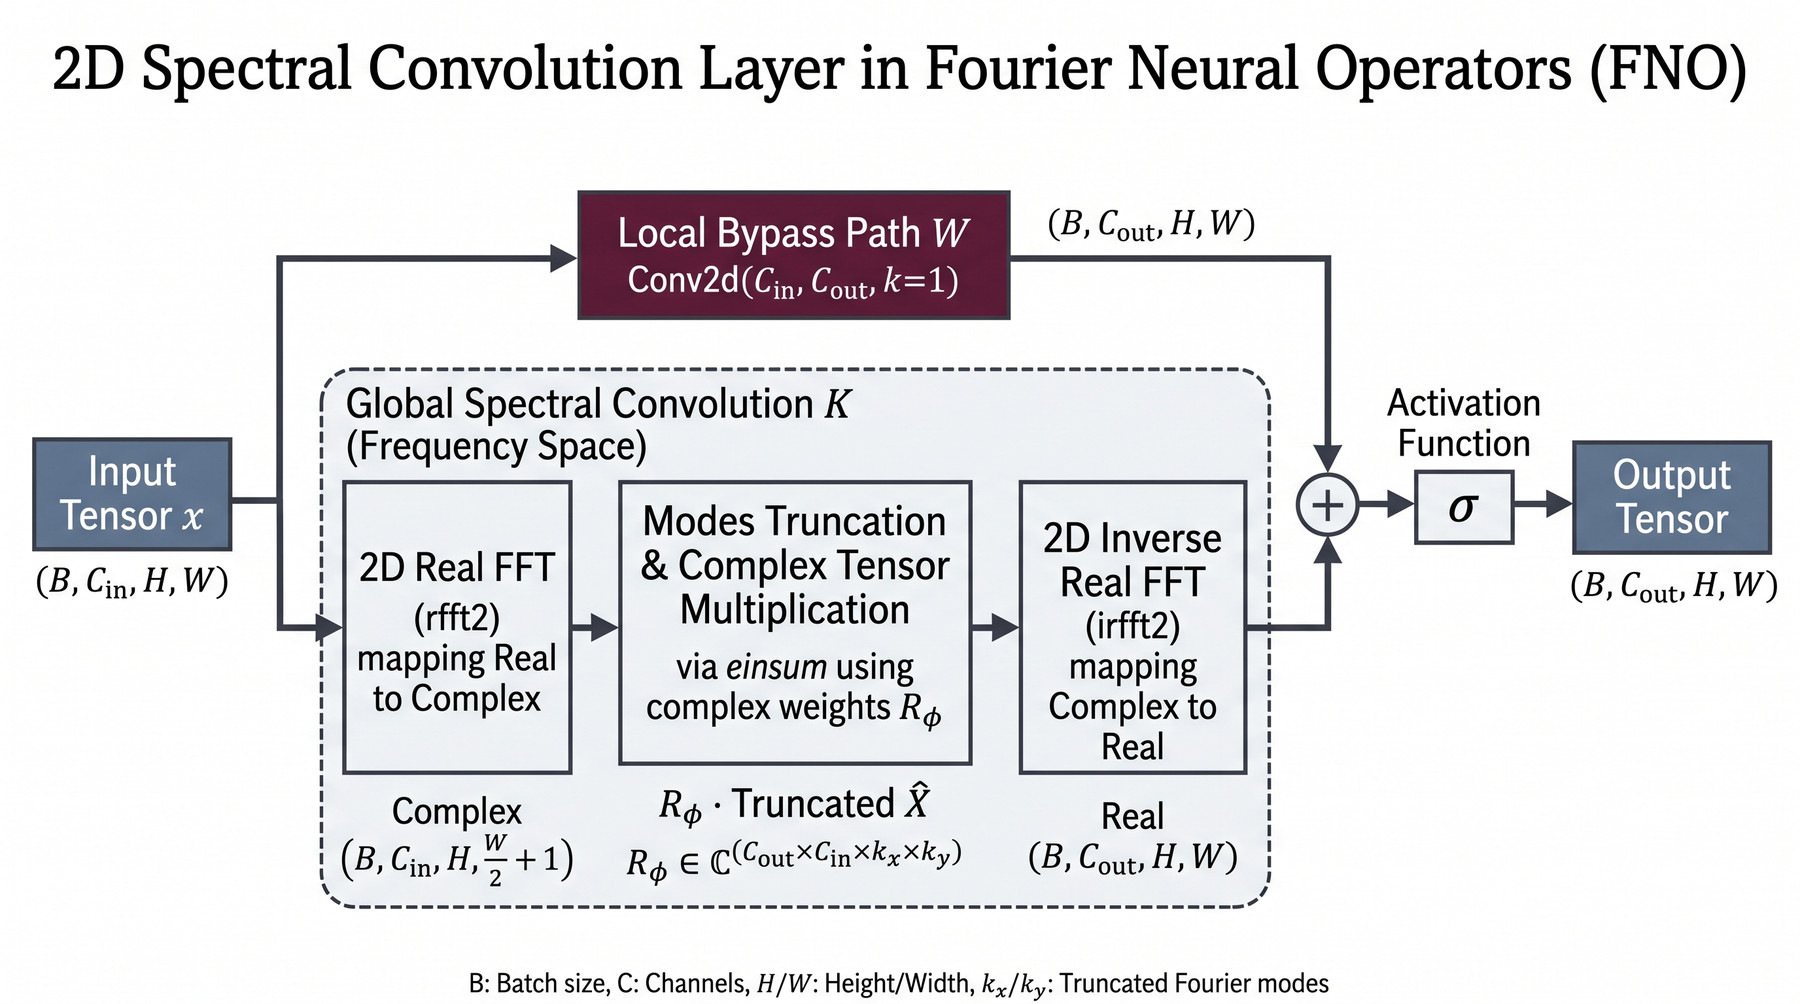
\includegraphics[width=0.95\textwidth]{fig_fno_spectral_layer.jpg}
\caption{\textbf{Architecture of the 2D Spectral Convolution Layer.} Input field $x$ splits into a local linear bypass $W x$ and a global spectral convolution $\mathcal{K} x$. The spectral branch computes the 2D real fast Fourier transform (FFT), slices the lowest $m_x \times m_y$ frequency modes, performs complex matrix multiplication via the learned parameter tensor $R_\phi$, zero-pads to the original grid shape, and reconstructs the physical representation via the inverse real FFT. Shapes at each stage are those of Listings~\ref{lst:ch23-spectral-conv2d} and~\ref{lst:ch23-fno2d}; the figure's legend denotes the retained mode counts by $k_x, k_y$, this book's text writes them $m_x, m_y$, and the code writes them \texttt{modes1}, \texttt{modes2}. The figure lists $R_\phi$ with the channel axes in the order $C_{\text{out}} \times C_{\text{in}}$; \eqref{eq:ch23-Rtensors} and the \texttt{einsum} subscript of Listing~\ref{lst:ch23-spectral-conv2d} fix the opposite order, and agree with each other.}
\label{fig:fno_spectral}
\end{figure}

Start with the transform. For a real input field
$x \in \mathbb{R}^{B \times C_{\text{in}} \times H \times W}$, its 2D
real-valued discrete Fourier transform is
\index{real-to-complex Fourier transform (rfft2)}
\begin{equation}
  \label{eq:ch23-rfft2}
  \hat{x} = \text{\texttt{torch.fft.rfft2}}(x) \in \mathbb{C}^{B \times C_{\text{in}} \times H \times (\lfloor W/2 \rfloor + 1)}.
\end{equation}
The call is the \emph{real-to-complex} FFT of the last two axes; the leading
batch and channel axes are carried along as transform batches, so one call
transforms the whole tensor rather than looping over fields. Two consequences
follow from the name. Because the input is real, conjugate symmetry holds:
$\hat{x}(-k_x, -k_y) = \overline{\hat{x}(k_x, k_y)}$, and the half-complex
representation in dimension $W$ fully determines the field --- the routine
returns $\lfloor W/2 \rfloor + 1$ coefficients along the last axis instead of
$W$, and the inverse \texttt{irfft2} reconstructs the omitted half from the
symmetry rather than from stored data. The second consequence is a budget
statement: a half-spectrum costs $2(\lfloor W/2 \rfloor + 1) \approx W$ real
values per row, which is what the real input already occupied, where a full
complex spectrum would cost twice that. Choosing \texttt{rfft2} over
\texttt{fft2} is therefore not a micro-optimization; it is what keeps the
frequency-domain intermediate no larger than the physical one.
\index{Fourier transform!real-to-complex, memory parity}

Parameterizing the convolution kernel begins by retaining the lowest $m_x$ and
$m_y$ modes. The retained set is a union of two contiguous blocks, called the
upper and lower corners in the comments of
Listing~\ref{lst:ch23-spectral-conv2d}:
\index{mode slicing!two-corner retention}
\begin{equation}
  \label{eq:ch23-corners}
  \begin{aligned}
  Z_m = \big\{(k_x, k_y): {}& k_x \in [0, m_x-1],\; k_y \in [0, m_y-1]\big\} \\
  \cup\; \big\{(k_x, k_y): {}& k_x \in [H - m_x, H-1],\; k_y \in [0, m_y-1]\big\}.
  \end{aligned}
\end{equation}
The two blocks are not ``low'' and ``high'' in the sense of one being more
oscillatory than the other. Under the usual ordering of FFT output, indices
$0, \dots, m_x - 1$ along the $H$ axis are the nonnegative small wavenumbers,
while indices $H - m_x, \dots, H - 1$ are the same wavenumbers taken with
negative sign; both are low in $|k_x|$. What makes the pair natural is
\eqref{eq:ch05-reality}: the conjugate of a mode with $k_y < 0$ is a mode with
$k_y > 0$, so storing the $k_y \ge 0$ half of the box and letting the inverse
transform supply the rest loses nothing. That is precisely the implementation
strategy Part~I announced when it observed that a real-output layer needs
weights for only half the modes and that this is the origin of two paired
weight tensors. The book-keeping is now explicit: \eqref{eq:ch23-corners} holds
$2 m_x m_y$ modes, against $(2m_x+1)(2m_y+1) \approx 4m_xm_y$ for the full box
$Z_{k_{\max}}$ of \eqref{eq:ch05-modeset}, and the factor of two is exactly the
one conjugacy buys, up to the self-conjugate line $k_y = 0$.

Two complex weight tensors are parameterized:
\begin{equation}
  \label{eq:ch23-Rtensors}
  R^{(1)} \in \mathbb{C}^{C_{\text{in}} \times C_{\text{out}} \times m_x \times m_y}, \qquad R^{(2)} \in \mathbb{C}^{C_{\text{in}} \times C_{\text{out}} \times m_x \times m_y}.
\end{equation}
\index{complex weight tensors}
Read \eqref{eq:ch23-Rtensors} against \eqref{eq:ch05-multiplier} and the
correspondence is one matrix per retained wavenumber: the continuum layer
carries $R_\phi(k) \in \mathbb{C}^{d_v \times d_v}$, and here those matrices
are stacked into two arrays whose last two indices enumerate the retained modes
of \eqref{eq:ch23-corners} and whose first two enumerate the channel rotation
applied at each of them. The one liberty is the order of those first two
indices: the arrays are stored with the input channel first, so each slice is
the transpose of the continuum matrix acting on a column of channel
coefficients. That convention is fixed by the \texttt{einsum} subscript below,
and it is the opposite of the one written on the figure. Note what is absent
from the shapes:
neither $H$ nor $W$ appears. The learnable parameters of a spectral layer do not
know the resolution they are applied to, which is the concrete form the
grid-independence of \eqref{eq:ch09-paramcount} takes in code.

Listing~\ref{lst:ch23-spectral-conv2d} is the complete layer. Its constructor
draws both arrays from a uniform distribution on $[0,1)$ scaled by
$1/(C_{\text{in}}C_{\text{out}})$ --- a small initialization, and an unusual one
in that its mean is positive. Every entry of every retained
mode therefore starts with the same sign, and the expected sum over input
channels at one output channel is
$C_{\text{in}}/(2C_{\text{in}}C_{\text{out}}) = 1/(2C_{\text{out}})$: on a
constant channel vector the spectral branch begins as a contraction, and must
learn its gain. In the forward pass, the line that
allocates
\texttt{out\_ft} as zeros is load-bearing twice over: it places the output
tensor on the input's device with the correct dtype, and it makes every mode
outside $Z_m$ identically zero, so the spectral branch is band-limited by
construction and truncation is a property of the data path rather than a penalty
term. The multiplication itself uses \texttt{torch.einsum} --- the Einstein
summation convention, in which a subscript appearing on both inputs and not on
the output is contracted --- with the pattern \texttt{"bixy,ioxy->boxy"}. The
letters name batch $b$, input channel $i$, output channel $o$, and the two mode
indices $x, y$; $i$ is summed, so at each retained mode $(x, y)$ the operation
is one matrix--vector product $C_{\text{out}} \times C_{\text{in}}$ against the
channel vector of coefficients at that mode. Nothing in the pattern carries a
term coupling $(x,y)$ to a different $(x',y')$, which is the code's version of
the diagonalization \eqref{eq:ch05-convolution-theorem} establishes.
\index{Einstein summation convention (einsum)}
\index{channel mixing!per-mode matrix product}

\begin{lstlisting}[language=Python, caption={\texttt{SpectralConv2d}: the 2D Fourier spectral convolution of \eqref{eq:ch23-rfft2}--\eqref{eq:ch23-Rtensors} in full. Its four commented stages map onto the three boxes of Figure~\ref{fig:fno_spectral}; the second stage, allocating the zeroed output tensor, is the zero-padding that figure's caption mentions rather than a box of its own.}, label={lst:ch23-spectral-conv2d}]
import torch
import torch.nn as nn

class SpectralConv2d(nn.Module):
    """2D Fourier Spectral Convolution Layer using complex matrix multiplication."""
    def __init__(self, in_channels: int, out_channels: int, modes1: int, modes2: int):
        super().__init__()
        self.in_channels = in_channels
        self.out_channels = out_channels
        self.modes1 = modes1 # Frequency modes along height H
        self.modes2 = modes2 # Frequency modes along width W

        # Complex weights initialized with uniform scaling
        scale = 1.0 / (in_channels * out_channels)
        self.weights1 = nn.Parameter(
            scale * torch.rand(in_channels, out_channels, self.modes1, self.modes2, dtype=torch.cfloat)
        )
        self.weights2 = nn.Parameter(
            scale * torch.rand(in_channels, out_channels, self.modes1, self.modes2, dtype=torch.cfloat)
        )

    def forward(self, x: torch.Tensor) -> torch.Tensor:
        # Input shape: (B, C_in, H, W)
        B, C, H, W = x.shape
        
        # 1. Compute 2D Real FFT: Output shape (B, C_in, H, W//2 + 1)
        x_ft = torch.fft.rfft2(x)
        
        # 2. Allocate complex output tensor in frequency domain
        out_ft = torch.zeros(B, self.out_channels, H, W // 2 + 1, device=x.device, dtype=torch.cfloat)
        
        # 3. Multiply retained Fourier modes by complex weight tensors
        # Upper corner: kx in [0, modes1), ky in [0, modes2)
        out_ft[:, :, :self.modes1, :self.modes2] = torch.einsum(
            "bixy,ioxy->boxy", x_ft[:, :, :self.modes1, :self.modes2], self.weights1
        )
        # Lower corner: kx in [-modes1, 0), ky in [0, modes2)
        out_ft[:, :, -self.modes1:, :self.modes2] = torch.einsum(
            "bixy,ioxy->boxy", x_ft[:, :, -self.modes1:, :self.modes2], self.weights2
        )
        
        # 4. Compute 2D Inverse Real FFT to return to physical domain
        x_out = torch.fft.irfft2(out_ft, s=(H, W))
        return x_out
\end{lstlisting}

% -----------------------------------------------------------------------------
\section{Cost, Parameter Count, and Failure Behavior of the Layer}
\label{sec:ch23-cost-and-failure}
% -----------------------------------------------------------------------------

Two remarks on the last line of Listing~\ref{lst:ch23-spectral-conv2d} before the
cost tally. The first concerns
resolution, and it does not come from the argument \texttt{s} but from the line
that reads \texttt{B, C, H, W} off the incoming tensor: every index in
\eqref{eq:ch23-corners} addresses a \emph{mode}, not a grid point, so handing the
same weights a $256 \times 256$ field evaluates the same band-limited multiplier
on a finer set of nodes. That is the code path behind
Proposition~\ref{prop:ch06-zeroshot}, with its caveat intact --- the identity is
exact for inputs already resolved on the training grid, and for nothing else.
The role of \texttt{s=(H, W)} is narrower and easily misread: a half-spectrum
with $\lfloor W/2 \rfloor + 1$ columns is compatible with two input widths, one
even and one odd, so the target shape has to be stated rather than inferred.
The second remark concerns normalization. PyTorch's forward transform is
unnormalized and its inverse divides by
$HW$, and the two factors cancel exactly across the pair. The learned array is
therefore the continuum multiplier $R_\phi(k)$ of \eqref{eq:ch05-multiplier},
apart from the transposition noted after \eqref{eq:ch23-Rtensors}, and not $HW$
times it; no grid-dependent rescaling of the weights is needed when the
grid changes, which is the numerical reason the parameter vector means the same
object on every mesh.

Counting operations per layer, for a batch of $B$ fields on an $H \times W$
grid,
\begin{equation}
  \label{eq:ch23-cost}
  \underbrace{5\,B\,(C_{\text{in}} + C_{\text{out}})\,HW \log_2(HW)}_{\text{forward and inverse transforms}}
  \;+\;
  \underbrace{6 \cdot 2\, B\, m_x m_y\, C_{\text{in}} C_{\text{out}}}_{\text{complex multiply--adds on } Z_m}
  \quad \text{floating-point operations},
\end{equation}
where $5N\log_2 N$ is the customary estimate for one complex transform of $N$
points, charged once over the $B C_{\text{in}}$ fields going in and once over
the $B C_{\text{out}}$ coming out, on an $H \times W$ array whose row and column
passes together give $\log_2 H + \log_2 W = \log_2(HW)$; and where a complex
multiply--add costs six real operations over the $2m_xm_y$ retained modes of
\eqref{eq:ch23-corners}. The first term overstates the real-to-complex pair by
roughly a factor of two, since a transform with a real input does about half the
work of a complex one of the same size; it is left in that form so that the
comparison below is conservative.
\index{computational cost!spectral layer, per-term}
Equation \eqref{eq:ch23-cost} is the operational content of the FNO line of
\eqref{eq:ch8-costs}, $\Theta(d_v N \log N + K d_v^2)$, with $K = 2m_xm_y$. Its
two halves behave very differently under refinement, and that asymmetry is the
argument: the learned arithmetic is the second term, which does not grow with
$H$ or $W$ at all, so refining the grid from $64^2$ to $256^2$ multiplies the
transform term by about $21$ --- a little more than the factor of $16$ in points,
because of the logarithm --- against the $256$ a dense discretization of
\eqref{eq:fredholm_kernel} would demand. At $64^2$ with $32$ channels and a
$12 \times 12$ band, the multiplier performs
$2 \cdot 144 \cdot 32 \cdot 32 \approx 3 \times 10^{5}$ complex multiply--adds
per field, while the dense alternative stores and applies an
$(HW)^2 \approx 1.7 \times 10^{7}$ kernel array per channel pair. The
$\mathcal{O}(N \log N)$ of
\chapref{ch:part1-the-fourier-neural-operator-spectral-theor} has become an
addressable object: it is the first term, and everything learnable sits in the
second.

The parameter count follows from \eqref{eq:ch23-Rtensors} directly,
\begin{equation}
  \label{eq:ch23-paramcount}
  P_{\text{spec}} = 2\, m_x m_y\, C_{\text{in}} C_{\text{out}} \ \text{complex} = 4\, m_x m_y\, C_{\text{in}} C_{\text{out}} \ \text{real}.
\end{equation}
For the reference two-dimensional configuration --- width
$C_{\text{in}} = C_{\text{out}} = 32$, band $m_x = m_y = 12$, depth $4$ ---
\eqref{eq:ch23-paramcount} gives $5.9 \times 10^{5}$ real numbers per spectral
layer and $2.4 \times 10^{6}$ across the stack: a few million parameters, set
entirely by the band and the width, with no term in $H$ or $W$ anywhere. The same
arithmetic explains why mode counts in practice sit at a dozen to sixteen per
direction: past the point where the algebraic truncation curve of
Figure~\ref{fig:spectral_decay} falls below the network's own error --- a term
that figure computes nothing about ---
widening $Z_m$ adds parameters without adding accuracy.
\index{parameter count!of a spectral layer}
\index{mode budget!reference configuration}

What breaks, and how loudly? The slicing convention of
\eqref{eq:ch23-corners} is the fragile part. If \texttt{modes2} exceeds
$\lfloor W/2 \rfloor + 1$, the slice returns fewer columns than
\texttt{weights1} has and \texttt{einsum} raises a shape error --- a loud,
immediately diagnosable failure. If instead $2\,\texttt{modes1} > H$ while
$\texttt{modes1} \le H$, both slices are well-formed, they overlap on the rows
$[H - \texttt{modes1},\, \texttt{modes1})$, and the second assignment silently
overwrites the first there. The layer still runs, still returns a tensor of the
right shape, and no longer computes the multiplier intended on the overlapping
modes. The safeguard is a constraint, not a check: keep $2m_x < H$ and
$m_y \le \lfloor W/2 \rfloor + 1$, which is the Nyquist-type hypothesis
$N_{\text{train}} > 2k_{\max}$ of Proposition~\ref{prop:ch06-zeroshot}
reappearing as a sanity bound on a configuration file.
\index{index slicing!overlap failure}

% -----------------------------------------------------------------------------
\section{Full FNO-2D Model Architecture}
\label{sec:ch23-fno2d}
% -----------------------------------------------------------------------------

The spectral layer is one stage of a network. Written as an operator on grid
fields, the assembled model is the discrete reading of \eqref{eq:fno_layer}
together with the composition \eqref{eq:no_composition}:
with $\mathcal{F}_N$ and $\mathcal{F}_N^{-1}$ the transform pair of
\eqref{eq:ch23-rfft2} and $R_\phi^{(N)}$ supported on $Z_m$ as in
\eqref{eq:ch23-corners},
\begin{equation}
  \label{eq:ch23-layer}
  v_{\ell+1} = \sigma\Big( W_\ell v_\ell + \mathcal{F}_N^{-1}\big( R_\phi^{(N)} \odot \mathcal{F}_N v_\ell \big) \Big),
  \qquad
  \mathcal{G}_\theta = \mathcal{Q} \circ \mathcal{V}^{(N)}_L \circ \cdots \circ \mathcal{V}^{(N)}_1 \circ \mathcal{P},
\end{equation}
where $\mathcal{V}^{(N)}_\ell$ is the map the left-hand display defines, taking
grid samples of $v_\ell$ to grid samples of $v_{\ell+1}$.
\index{FNO-2D!layer recursion}
The full network wraps the spectral convolutions between a local lifting
multilayer perceptron (MLP) $\mathcal{P}$ and a projection MLP $\mathcal{Q}$, and
Listing~\ref{lst:ch23-fno2d} is that construction in full. Three details of the
listing carry the design.

\begin{lstlisting}[language=Python, caption={The complete FNO-2D of \eqref{eq:ch23-layer}: grid embedding, pointwise lifting, a stack of spectral blocks with local bypass, and pointwise projection.}, label={lst:ch23-fno2d}]
class FNO2d(nn.Module):
    """Full 2D Fourier Neural Operator with stacked spectral-convolution layers."""
    def __init__(self, in_channels: int, out_channels: int, modes1: int, modes2: int, 
                 hidden_channels: int = 32, n_layers: int = 4):
        super().__init__()
        self.grid_embed = GridEmbeddingND(dim=2)
        
        # Lifting: maps (C_in + 2) channels to hidden dimension
        self.p = nn.Conv2d(in_channels + 2, hidden_channels, kernel_size=1)
        
        # Stack of Fourier operator layers
        self.spectral_layers = nn.ModuleList([
            SpectralConv2d(hidden_channels, hidden_channels, modes1, modes2)
            for _ in range(n_layers)
        ])
        self.ws = nn.ModuleList([
            nn.Conv2d(hidden_channels, hidden_channels, kernel_size=1)
            for _ in range(n_layers)
        ])
        
        # Projection: maps hidden dimension back to C_out channels
        self.q = nn.Sequential(
            nn.Conv2d(hidden_channels, 128, kernel_size=1),
            nn.GELU(),
            nn.Conv2d(128, out_channels, kernel_size=1)
        )
        self.act = nn.GELU()

    def forward(self, x: torch.Tensor) -> torch.Tensor:
        # Append positional grid coordinates
        x = self.grid_embed(x)
        x = self.p(x) # Shape: (B, hidden_channels, H, W)
        
        for spec_conv, w_conv in zip(self.spectral_layers, self.ws):
            # Parallel spectral and local bypass paths
            x1 = spec_conv(x)
            x2 = w_conv(x)
            x = self.act(x1 + x2)
            
        x = self.q(x) # Shape: (B, out_channels, H, W)
        return x
\end{lstlisting}

First, the lifting convolution takes \texttt{in\_channels + 2} inputs. The extra
two are the normalized coordinate channels appended by \texttt{GridEmbeddingND},
the utility of \chapref{ch:part2-the-practitioner-s-paradigm-infinite-dimen}
that turns a field into $a_{\text{augmented}} = [a, x_1, x_2]$.
\index{coordinate channels!in FNO lifting}
The consequence is easy to misdescribe.
The coordinate channels are not carried through as geometry: lifting mixes them
into the hidden channels, and from that point on they are transformed and
truncated like everything else. What they contribute is a location. Every
operation in \eqref{eq:ch23-layer} is equivariant to translations on the torus
--- that is precisely what the diagonalization \eqref{eq:ch05-convolution-theorem}
buys --- so a network fed only field values cannot distinguish a feature at $x$
from the same feature at $x + h$. Appending $x_1$ and $x_2$ is the cheap way to
break that symmetry, and it is the translational ambiguity of
\chapref{ch:part2-the-practitioner-s-paradigm-infinite-dimen} seen from the
inside of a forward pass.

Second, both $\mathcal{P}$ and $\mathcal{Q}$ are built from $1 \times 1$
convolutions, which are pointwise maps. The lift in the listing is a single such
convolution --- the degenerate case of the shallow MLP that
\eqref{eq:no_composition} permits --- while the projection is a two-layer
stack, $C_{\text{hid}} \to 128 \to C_{\text{out}}$ through a Gaussian error
linear unit (GELU). Both act independently at every grid point, so all spatial
communication in the model happens in the spectral branch or in the bypass, and
the input and output resolutions are identical --- the network is grid-to-grid,
and no interpolation stage appears anywhere in \eqref{eq:ch23-layer}.

Third, and most substantive: why keep $W_\ell$ at all, when the spectral branch
already performs a global learned operation? The answer is a limitation of
\eqref{eq:ch23-layer} that the code makes visible. The spectral branch maps its
input into the band-limited subspace spanned by $Z_m$ and discards everything
else; the pointwise $W_\ell$ is the only path by which content outside the band
reaches layer $\ell + 1$ intact. Without it, information above the cutoff could
survive only by being folded down through the nonlinearity --- $\sigma$ applied
to a band-limited field generates harmonics outside the band, which the next
layer truncates again --- a lossy and poorly controlled route. The bypass is thus
the price of truncation, not redundancy: it is what lets a twelve-mode layer
still be a map on fields rather than a map on twelve-mode
approximations.
\index{local bypass convolution!necessity}

Grid-independence also fixes the bias. \chapref{ch:part1-the-fourier-neural-operator-spectral-theor}
writes \eqref{eq:fno_layer} with a bias $b_\ell(x)$ that is a function of
position. In the listing, the bias is the default \texttt{bias} of
\texttt{nn.Conv2d}: one constant per output channel, shared across all $HW$
locations. That is a deliberate specialization, and a necessary one. A bias
attached to grid points would add $HW$ learnable numbers per channel, the
parameter array would acquire a shape dependent on the discretization, and the
grid-independence visible in \eqref{eq:ch23-Rtensors} --- and asserted by
\eqref{eq:ch09-paramcount} --- would be forfeited. Part~I excludes such an
architecture on exactly those grounds; here is the exclusion implemented.
\index{bias!pointwise versus grid-attached}

Tracing shapes through the forward pass fixes the rest of the accounting. A batch
of scalar fields arrives as $(B, 1, H, W)$, becomes $(B, 3, H, W)$ after grid
embedding, $(B, C_{\text{hid}}, H, W)$ after lifting, and stays at
$(B, C_{\text{hid}}, H, W)$ through all $L$ blocks --- the architecture is a
width-preserving stack with no pooling, no striding, and no upsampling, which is
what distinguishes it structurally from a convolutional encoder--decoder.
Each block holds a spectral array counted by \eqref{eq:ch23-paramcount} and a
bypass of $C_{\text{hid}}^2 + C_{\text{hid}}$ parameters, so at
$C_{\text{hid}} = 32$
the bypass contributes under one percent of the block's parameters while
contributing all of its spatially unresolved behavior. Memory, however, follows
the frequency tensor, not the parameter count: at $B = 16$,
$C_{\text{hid}} = 32$ and $H = W = 64$, both \texttt{x\_ft} and
\texttt{out\_ft} occupy $16 \cdot 32 \cdot 64 \cdot 33 \approx 1.1 \times 10^{6}$
complex entries, about $8.7$ MB in fp32-complex each, and an autograd-enabled
forward pass retains both per layer --- roughly $70$ MB of frequency-domain
intermediates for a four-layer stack before counting anything else. Those are
fp32 figures; the case for running parts of the network in bfloat16, and the
reason the transform and the complex multiplication are the last places one
applies automatic mixed precision (AMP), is taken up in
\chapref{ch:part2-training-regimes-optimization-and-failure-}.
\index{memory footprint!frequency-domain intermediates}
\index{automatic mixed precision (AMP)}

% -----------------------------------------------------------------------------
\section{Using the Official \texttt{neuraloperator} Library}
\label{sec:ch23-library}
% -----------------------------------------------------------------------------

Everything above is under a hundred lines of PyTorch, and a reader should be
able to write it, read it, and debug it. Production use is a different matter.
The official \texttt{neuraloperator} library maintained by Caltech and NVIDIA
provides industrial-grade implementations, including a factorized variant --- the
\texttt{TFNO} class that the workflow of
Listing~\ref{lst:ch23-neuraloperator-workflow} instantiates --- in which the
multiplier arrays of \eqref{eq:ch23-Rtensors} are stored through a Tucker or
CANDECOMP/PARAFAC (CP) tensor decomposition instead of as dense arrays, which
compresses the parameter store without changing the arithmetic of
\eqref{eq:ch23-layer}.
\index{neuraloperator library}
\index{tensor factorization!of spectral multiplier arrays}
\index{CANDECOMP/PARAFAC (CP) decomposition}

The mechanism of that compression is worth stating, because it is the one place
where the library departs from the parameterization \eqref{eq:ch23-Rtensors} in
a way that earns its keep. \eqref{eq:ch23-Rtensors} stores the mode-indexed channel
rotations as a four-way array and spends \eqref{eq:ch23-paramcount} parameters
on it; a Tucker decomposition replaces the array by a small core tensor
contracted with one factor matrix along each axis, and a
CP decomposition replaces it by a sum of rank-one terms
\index{Tucker decomposition!in a factorized spectral layer}
--- the multilinear reconstruction \eqref{eq:ch8-tucker} of
\chapref{ch:part1-comparative-theoretical-taxonomy-of-archit}, drawn there with
the mode index flattened into a single axis and four-way here because
\eqref{eq:ch23-Rtensors} keeps the two spatial mode axes distinct. What changes
is which products appear. \eqref{eq:ch8-tucker} costs a term linear in the band
size times the mode rank, plus terms linear in each channel width, where
\eqref{eq:ch23-paramcount} pays the band size times \emph{both} channel widths
at once; widening the band --- which is what buys accuracy when the target's
regularity is low, per \eqref{eq:ch05-error-decomposition} --- therefore costs
one extra rank's worth of parameters per mode instead of
$C_{\text{in}}C_{\text{out}}$ worth. How much any particular configuration saves
is thus fixed by the rank chosen against the band and the channel widths entered
in \eqref{eq:ch23-paramcount}, not by the factorization as such: the two counts
can be subtracted by hand on any configuration, and the \texttt{rank=0.42} of
Listing~\ref{lst:ch23-neuraloperator-workflow} is one illustration of the
trade; the percentage annotated on that line describes
that example alone and is not a compression factor this book reports. Compression is not free, however, and Part~I is explicit about
the price: the ranks must genuinely be small for the count to fall, and whether
the multiplier arrays a solution operator induces are low-rank is an empirical
premise that no theorem here supports. Factorizing constrains
\eqref{eq:ch23-Rtensors} to a low-rank manifold that
\eqref{eq:ch05-error-decomposition} does not account for, so band and rank trade
off in a way the theory leaves to the validation curve.

\begin{lstlisting}[language=Python, caption={The canonical training workflow of the official \texttt{neuraloperator} library: a factorized model, the relative-$L^p$ loss, and the optimizer, assembled as three independent objects.}, label={lst:ch23-neuraloperator-workflow}]
from neuralop.models import FNO, TFNO
from neuralop import LpLoss
from neuralop.training import AdamW

# Instantiate Tensorized FNO (TFNO) for high memory efficiency
model = TFNO(
    n_modes=(16, 16),
    in_channels=1,
    out_channels=1,
    hidden_channels=64,
    factorization='tucker',
    rank=0.42 # Compresses complex parameter tensor by 58%
).cuda()

loss_fn = LpLoss(d=2, p=2)
optimizer = AdamW(model.parameters(), lr=8e-3, weight_decay=1e-4)
\end{lstlisting}

Listing~\ref{lst:ch23-neuraloperator-workflow} is the workflow, and comparing it
line by line with Listings~\ref{lst:ch23-spectral-conv2d}
and~\ref{lst:ch23-fno2d} shows what the library keeps and what it changes. The
object model is the same. The pair \texttt{modes1} and \texttt{modes2} reappears
as \texttt{n\_modes}, the hidden width keeps the name \texttt{hidden\_channels},
and the input and output channel counts are both $1$ --- the Darcy
coefficient-to-pressure map of \eqref{eq:darcy}, scalar input, scalar output,
same grid in and out. What the library adds is the machinery a from-scratch file
leaves implicit: the factorization keyword, device placement made explicit by a
\texttt{.cuda()} call on the whole module, and a loss and an optimizer that
arrive as separate objects. Two of those differences bear on the computation.
The library's \texttt{LpLoss} takes an
explicit spatial-dimension argument \texttt{d=2}, because it forms a
quadrature-weighted norm of the kind in \eqref{eq:rel_l2_loss} rather than a
plain vector norm over flattened data; on an equispaced grid the weights cancel
in the ratio and the two coincide, which is exactly why the from-scratch version
of \chapref{ch:part2-the-practitioner-s-paradigm-infinite-dimen} is safe there.
A weighted implementation keeps its meaning when the quadrature is nonuniform
or when the norm mixes terms of different differential order. And
\texttt{AdamW} --- Adam with decoupled weight decay --- is imported from the library's own training module, though \texttt{torch.optim}
provides its own implementation, so that a question the from-scratch file never has
to answer is settled
once, for every user:
what decay applied to the complex arrays of \eqref{eq:ch23-Rtensors} acts on,
their magnitudes or their real and imaginary parts separately.
\index{AdamW optimizer}
\index{relative $L^2$ loss!quadrature-weighted variant}

The learning rate of \texttt{lr=8e-3} should be read with care. It is an initial
value, not a recommendation to train at a constant rate: because complex
Fourier multipliers act directly on the frequency modes, holding a rate of this
size fixed produces early training instability, and the schedule that makes such
a rate usable --- one-cycle ramping, gradient clipping, and the weight decay
already visible above --- is the subject of
\chapref{ch:part2-training-regimes-optimization-and-failure-}. Likewise, the
model returned by \texttt{TFNO(...).cuda()} is trained and evaluated by exactly
the arithmetic of \eqref{eq:ch23-layer}; what the library does not do is choose
the band. That choice, made in \eqref{eq:ch23-corners} and argued in
\chapref{ch:part1-the-fourier-neural-operator-spectral-theor}, remains the
practitioner's, and it remains the single hyperparameter whose effect on accuracy
the theory actually predicts.
\index{hyperparameters!mode budget as the predicted one}

% -----------------------------------------------------------------------------
\medskip
The layer written here buys its $\mathcal{O}(N \log N)$ cost with three
purchases: a periodic torus, a stationary kernel, and a fixed band. The first is
the binding one for everything this book will later simulate. External
aerodynamics over a car body, flow through a faulted porous reservoir, and
electrophysiology on a ventricle do not live on $[0,1)^2$, and no amount of
padding or masking makes a tensor-product grid conform to a boundary that curves
through it. \index{Fourier neural operator!limitations of, periodic domains}
Neither is the truncation of \eqref{eq:ch23-corners} available, since on an
unstructured mesh there is no transform whose output axes a slice could address.
\chapref{ch:part2-graph-neural-operators-gno-and-irregular-g}
therefore abandons diagonalization and returns to the Fredholm kernel
\eqref{eq:fredholm_kernel} in its unspecialized form, evaluating it by local
quadrature over neighborhoods rather than globally over frequencies: the graph
neural operator (GNO), whose per-layer cost $\Theta(|E| d_v^2)$ in
\eqref{eq:ch8-costs} is set by the number of mesh edges instead of the number of
grid points, and whose implementation is the subject of that chapter's first
half. The two architectures are not rivals but complements, and its second half
composes them: the geometry-informed neural operator (GINO) puts graph layers at
either end of a latent spectral stack, leaving the mesh, doing the fast global
work in frequency space, and returning.
